
\documentclass[11pt]{article}
% DOCUMENT COOKBOOK / SHARED SETUP. INPUT THIS FILE; DO NOT COMPILE IT.
% The ordinary document remains flowing text. Every optional feature below
% stays inactive unless explicitly used in a document or recipe.

% FOUNDATION: page geometry and typography
\usepackage[T1]{fontenc}
\usepackage{lmodern,microtype}
\usepackage[letterpaper,margin=1in]{geometry} % change paper/margins here
\usepackage{setspace}
\setlength{\parindent}{1.3em}
\setlength{\parskip}{0pt}

% Scientific writing and layout
\usepackage{amsmath,amssymb,amsthm,bm}
\usepackage{graphicx,caption,subcaption,wrapfig,float,placeins}
\usepackage{booktabs,tabularx,array,multicol}
\usepackage{xcolor,tikz}
\usetikzlibrary{calc,positioning}
\usepackage{titlesec}
\usepackage{fancyhdr}
\usepackage{listings}
\definecolor{CUGold}{HTML}{CFB87C}
\definecolor{Ink}{HTML}{193848}
\definecolor{Teal}{HTML}{237C89}
\definecolor{Muted}{HTML}{5E7179}
\definecolor{Soft}{HTML}{EFF5F6}
\graphicspath{{figures/}}
\captionsetup{font=small,labelfont=bf}
\newtheorem{theorem}{Theorem}[section]
\theoremstyle{definition}
\newtheorem{definition}[theorem]{Definition}
\lstset{basicstyle=\ttfamily\footnotesize,frame=single,breaklines=true,
  columns=fullflexible,keepspaces=true,showstringspaces=false,
  keywordstyle=\color{Teal},commentstyle=\color{Muted}}

% Citation system: biblatex + Biber. Do not mix with natbib/BibTeX commands.
\usepackage[backend=biber,style=numeric,sorting=none]{biblatex}
\addbibresource{references.bib}
\usepackage[colorlinks=true,linkcolor=Ink,citecolor=Teal,urlcolor=Teal]{hyperref}
\usepackage[noabbrev,nameinlink]{cleveref}

% FOUNDATION: customize an OPTIONAL precision-placed title page.
% First fontsize argument is the font size (pt); second is baseline spacing.
\newcommand{\DocTitleFont}{\color{Ink}\fontsize{25}{31}\selectfont\bfseries}
\newcommand{\DocSubtitleFont}{\color{Muted}\fontsize{14}{20}\selectfont}
\newcommand{\DocAuthorFont}{\color{Ink}\fontsize{13}{18}\selectfont}
\newcommand{\DocAffiliationFont}{\color{Muted}\fontsize{11}{15}\selectfont}

% PAGE coordinates: X from page left, Y downward from page top (cm).
% Page objects are overlays: they occupy NO flow space; use on title pages.
% \DocPageTextAt{X}{Y}{WIDTH}{TEXT}
\newcommand{\DocPageTextAt}[4]{%
  \begin{tikzpicture}[remember picture,overlay]
    \node[anchor=north west,inner sep=0pt,outer sep=0pt]
      at ([xshift=#1cm,yshift=-#2cm]current page.north west) {%
        \begin{minipage}[t]{#3}\vspace{0pt}#4\par\end{minipage}};
  \end{tikzpicture}%
}
% \DocPageImageAt{X}{Y}{WIDTH}{FILE}
\newcommand{\DocPageImageAt}[4]{%
  \begin{tikzpicture}[remember picture,overlay]
    \node[anchor=north west,inner sep=0pt,outer sep=0pt]
      at ([xshift=#1cm,yshift=-#2cm]current page.north west)
      {\includegraphics[width=#3]{#4}};
  \end{tikzpicture}%
}

% CONTAINER-LOCAL coordinates: X right, Y down from the local TikZ origin.
% Place these ONLY within a tikzpicture (usually inside a figure/minipage).
% \DocImageAt{X}{Y}{WIDTH}{FILE}
\newcommand{\DocImageAt}[4]{%
  \node[anchor=north west,inner sep=0pt,outer sep=0pt] at (#1,-#2)
    {\includegraphics[width=#3]{#4}};%
}
% \DocTextAt{X}{Y}{WIDTH}{TEXT}
\newcommand{\DocTextAt}[4]{%
  \node[anchor=north west,inner sep=0pt,outer sep=0pt] at (#1,-#2) {%
    \begin{minipage}[t]{#3}\vspace{0pt}#4\par\end{minipage}};%
}
% \DocCanvas{WIDTH}{HEIGHT}{CONTENT}: explicit space, cm; no clipping.
\newcommand{\DocCanvas}[3]{%
  \begin{tikzpicture}[x=1cm,y=1cm]
    \useasboundingbox (0,0) rectangle (#1,-#2);
    #3
  \end{tikzpicture}%
}
% \DocAutoCanvas{CONTENT}: auto-sized bounding box; no reserved height.
\newcommand{\DocAutoCanvas}[1]{%
  \begin{tikzpicture}[x=1cm,y=1cm]
    \path (0,0);#1
  \end{tikzpicture}%
}

% OPT-IN REPEATED FOOTER. The blank document does NOT enable this.
% \DocSetFooter{LEFT}{CENTER}{RIGHT}{RULE THICKNESS}
\newcommand{\DocSetFooter}[4]{%
  \fancyhf{}\fancyfoot[L]{\footnotesize #1}
  \fancyfoot[C]{\footnotesize #2}\fancyfoot[R]{\footnotesize #3}
  \renewcommand{\headrulewidth}{0pt}%
  \renewcommand{\footrulewidth}{#4}%
  \pagestyle{fancy}%
}


\title{APPM 5460 Project Proposal}
\author{Chuan Wei Heng}
\date{\today}

\begin{document}
\maketitle

\section{Background}

This project is motivated by my ongoing research in
Professor Ankur Gupta's laboratory, where I investigate
the theoretical modeling of coupled multicomponent ion
transport in electrolyte systems. In particular, I
consider an aqueous electrolyte containing hydrogen
($H^+$), hydroxide ($OH^-$), sodium ($Na^+$), and
chloride ($Cl^-$) ions.

The transport of these species is governed by diffusion
and electromigration, with the ions coupled through
the electrostatic potential generated by their charge
distribution. In addition, hydrogen and hydroxide ions
undergo an acid--base neutralization reaction to form
water. The resulting system is described by the
Poisson--Nernst--Planck equations coupled to chemical
reaction kinetics.

\subsection*{Governing Equations}

The conservation equation for each ionic species is

\begin{equation}
    \frac{\partial c_i}{\partial t}
    = -\nabla\cdot\bm{J}_i + R_i,
    \qquad
    i \in \{H^+, OH^-, Na^+, Cl^-\},
    \label{eq:continuity}
\end{equation}

where $c_i$ denotes the concentration, $\bm{J}_i$
the molar flux, and $R_i$ the net rate of production
of species $i$.

The ionic flux is described by the Nernst--Planck
equation,

\begin{equation}
    \bm{J}_i
    = -D_i\left(
        \nabla c_i
        + \frac{z_i F}{RT}c_i\nabla\phi
    \right),
    \label{eq:nernst_planck}
\end{equation}

where $D_i$ and $z_i$ are the diffusivity and valence
of species $i$, respectively. Furthermore, $F$ is
Faraday's constant, $R$ is the ideal gas constant,
$T$ is the absolute temperature, and $\phi$ is the
electrostatic potential.

The acid--base reaction is modeled using the
following second-order reaction kinetics:

\begin{align}
    R_{H^+} = R_{OH^-}
    &= -kc_{H^+}c_{OH^-},
    \label{eq:reaction}\\
    R_{Na^+} = R_{Cl^-}
    &= 0.
\end{align}

Finally, the electrostatic potential is determined
self-consistently through Poisson's equation,

\begin{equation}
    -\varepsilon\nabla^2\phi
    = \rho_e
    = F\sum_i z_i c_i,
    \label{eq:poisson}
\end{equation}

where $\varepsilon$ denotes the permittivity
and $\rho_e$ is the local charge density.

\subsection*{Domain and Boundary Conditions}

We consider a one-dimensional domain of length $L$,
with prescribed ionic concentrations and electrostatic
potentials at both boundaries.

\begin{figure}[htbp]
    \centering
    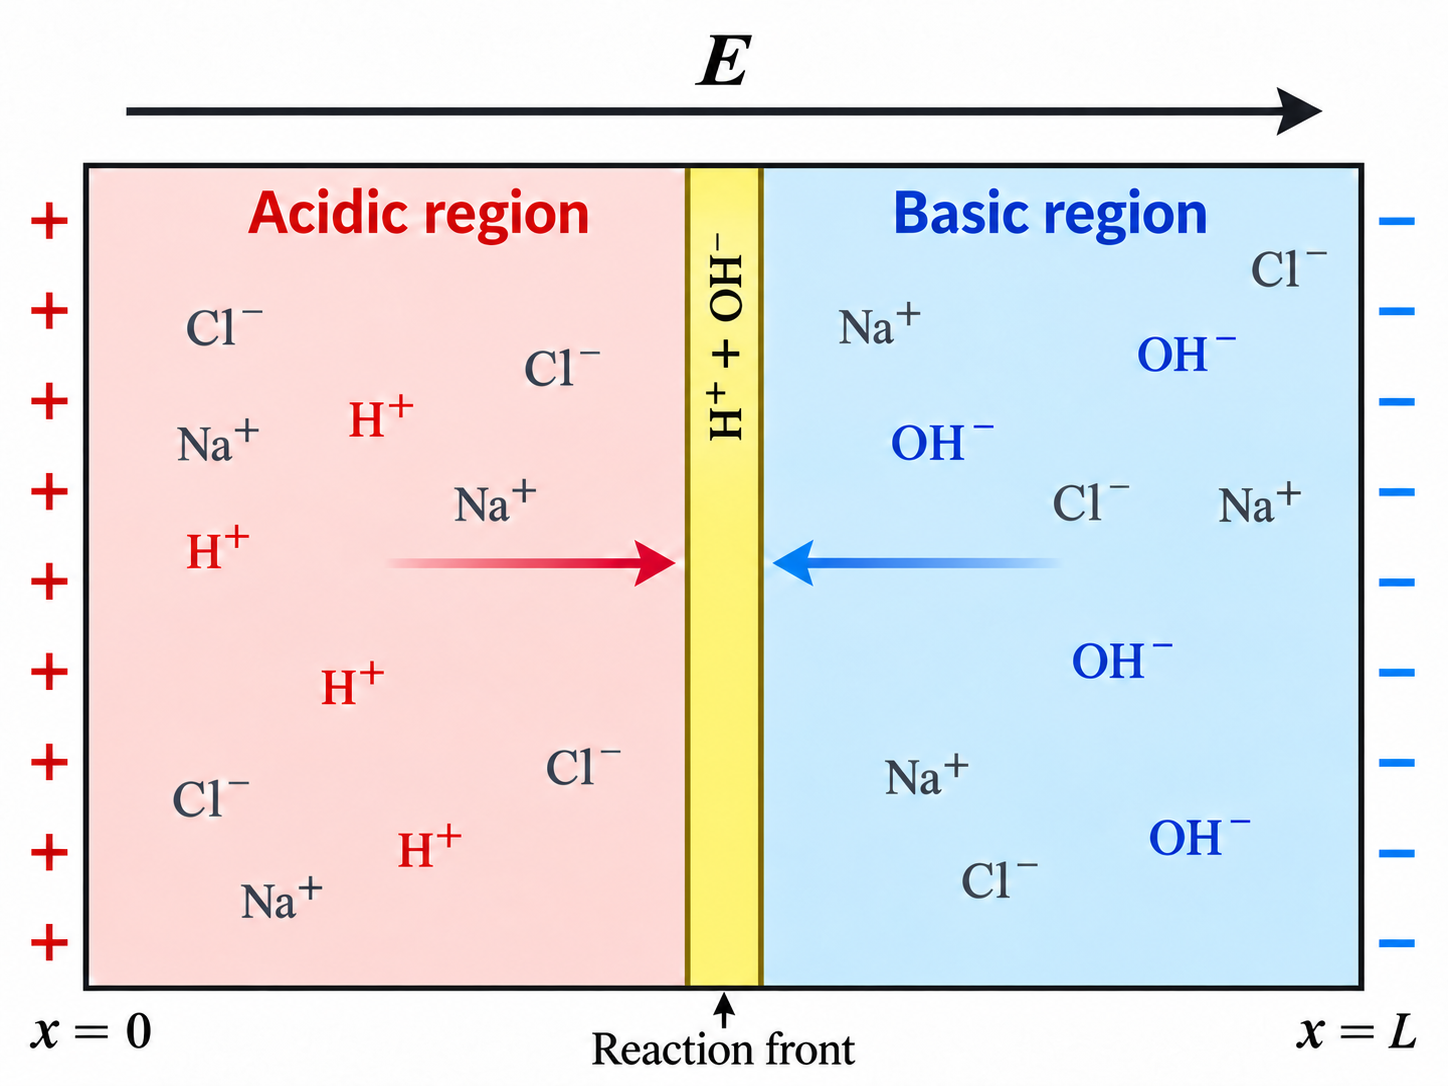
\includegraphics[width=0.65\textwidth]
        {figures/Electrochemical Reaction Front Diagram.png}
    \caption{Schematic of the one-dimensional
    electrolyte domain and acid--base reaction front.}
    \label{fig:reaction_front_domain}
\end{figure}

At the left boundary, $x=0$,

\begin{equation}
    \begin{aligned}
        c_{H^+} &= c_0,
        &\qquad c_{Na^+} &= c_s,\\
        c_{OH^-} &= 0,
        &\qquad c_{Cl^-} &= c_0+c_s,\\
        \phi &= \phi_0.
    \end{aligned}
    \label{eq:bc_left}
\end{equation}

At the right boundary, $x=L$,

\begin{equation}
    \begin{aligned}
        c_{H^+} &= 0,
        &\qquad c_{Cl^-} &= 0,\\
        c_{Na^+} &= c_0,
        &\qquad c_{OH^-} &= c_0,\\
        \phi &= \phi_L.
    \end{aligned}
    \label{eq:bc_right}
\end{equation}

The initial ionic concentrations in the interior
of the domain are prescribed as

\begin{equation}
    c_i(x,0)=0,
    \qquad 0<x<L,
    \qquad \forall i.
    \label{eq:initial}
\end{equation}


\section{Electroosmotic Instabilities}

Our recent research has led us to hypothesize that
electroconvective vortices may develop near an acid--base
reaction front under an externally applied electric
potential. This hypothesis is motivated by earlier work
on electroconvective instabilities near ion-selective
membranes, particularly the work of
\textcite{rubinstein2000electro}.

In these systems, electrokinetic instabilities can
generate vortical fluid motion near the membrane
interface. This phenomenon is commonly associated
with the Rubinstein--Zaltzman instability.

\begin{figure}[htbp]
    \centering
    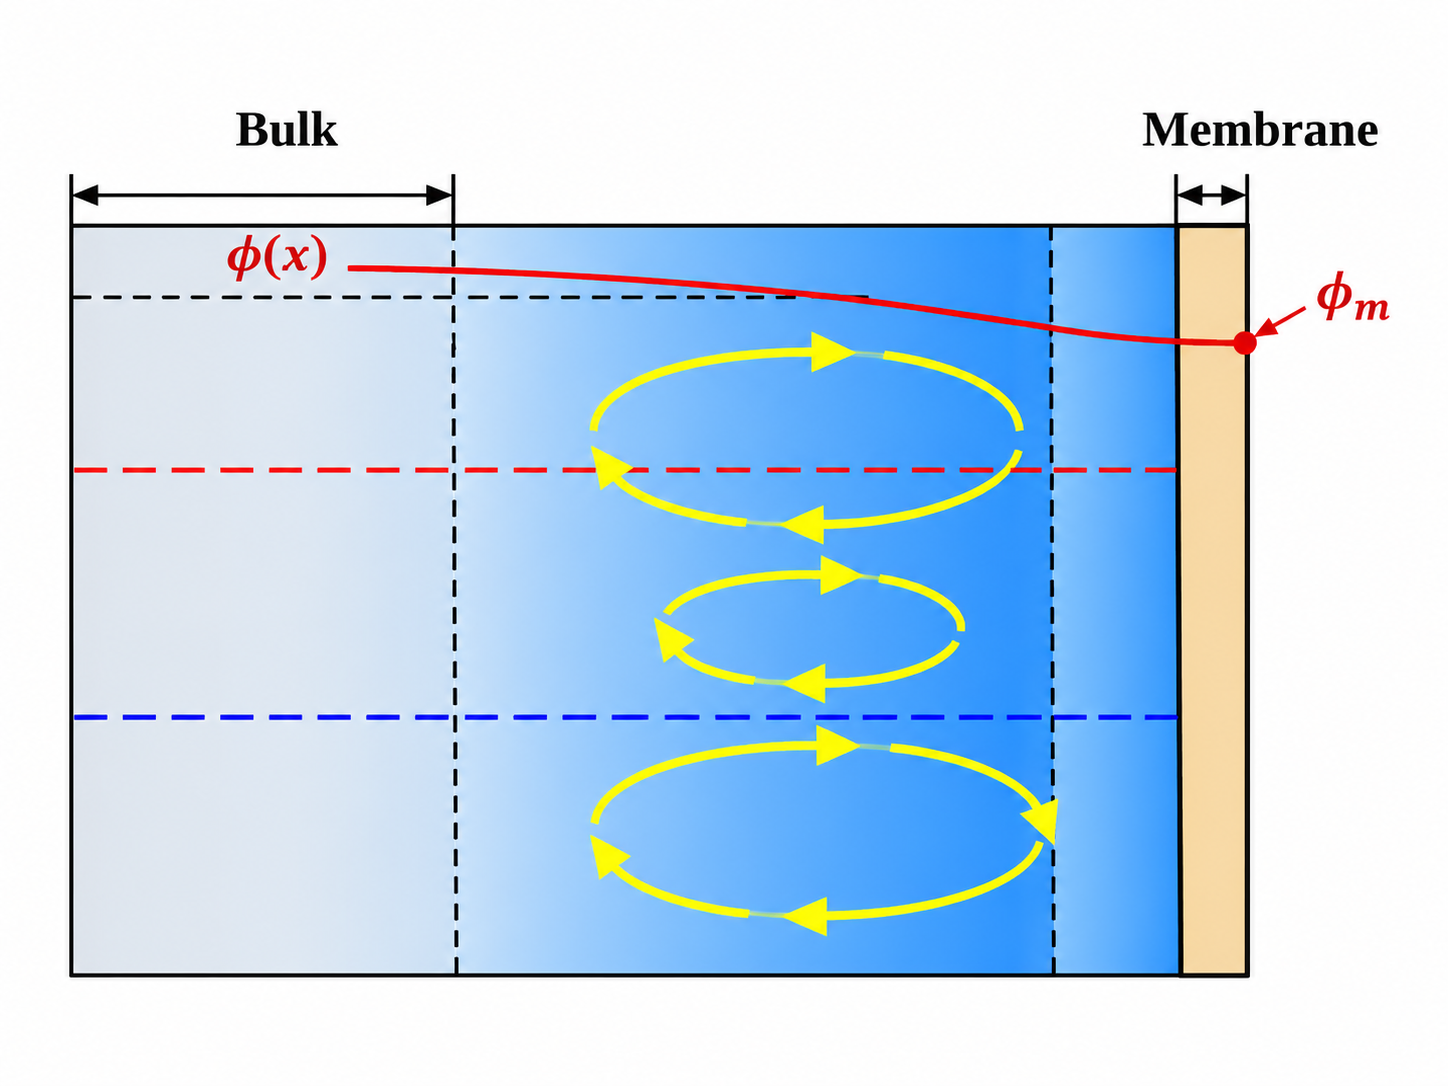
\includegraphics[width=0.65\textwidth]
        {figures/membrane_vortex.png}
    \caption{Schematic of electroconvective vortices
    near the interface of an ion-selective membrane.}
    \label{fig:membrane_vortices}
\end{figure}

Inspired by this mechanism, we seek to investigate
whether a related instability can arise in a
membraneless electrolyte system, where the acid--base
reaction front creates spatial variations in ionic
concentrations and electrical properties.

Unlike membrane-based systems, the proposed instability
would occur without a physical ion-selective interface.
Consequently, the existence and underlying mechanism
of such an instability remain to be established.

Our central research question is therefore:
\textit{Can a Rubinstein--Zaltzman-type electroconvective
instability arise near a membraneless acid--base
reaction front?}

\begin{figure}[htbp]
    \centering
    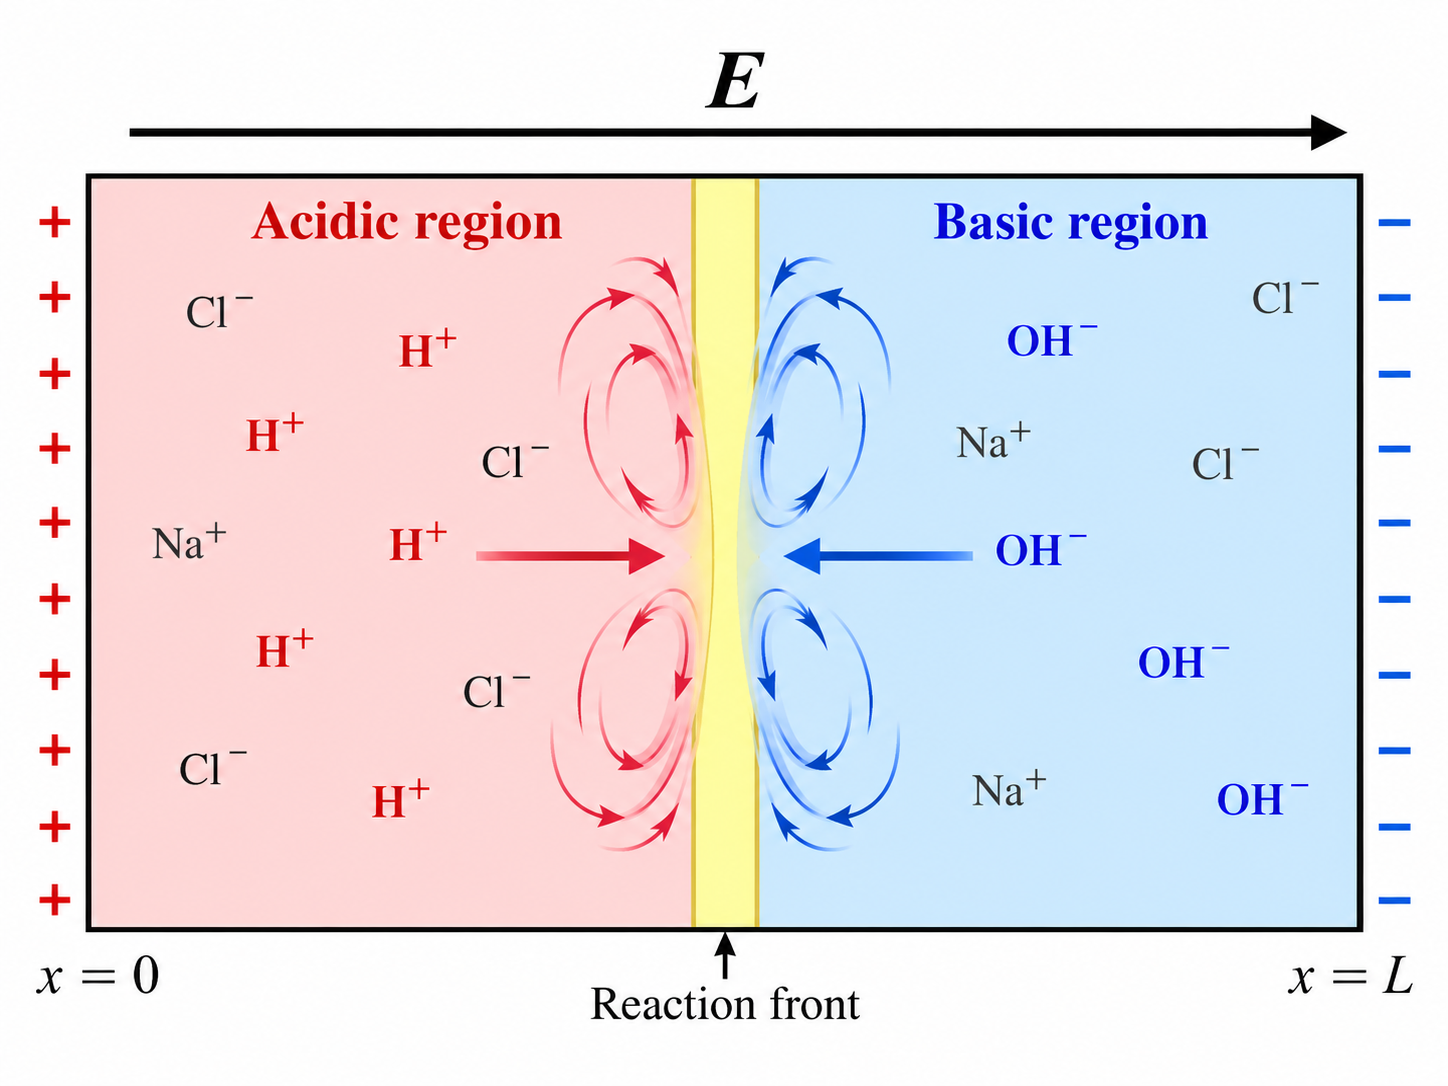
\includegraphics[width=0.65\textwidth]
        {figures/membraneless_vortex.png}
    \caption{Schematic of hypothesized electroconvective
    vortices near a membraneless acid--base reaction
    front under an applied electric potential.}
    \label{fig:membraneless_vortices}
\end{figure}


\section{Proposed Investigation}

The objective of this project is to investigate the
dynamical stability of the coupled ion-transport system
and determine whether electroconvective instabilities
can arise under an applied electric potential.

We propose to begin by examining the steady-state
solutions of the one-dimensional
Poisson--Nernst--Planck--reaction system, which
will serve as the base state for our stability
analysis. Particular attention will be given to
the spatial distributions of ionic concentrations,
electric potential, and charge density near the
reaction front.

We will then consider extending the model to
incorporate fluid motion and investigate the
response of the base state to small perturbations.
By linearizing the governing equations about the
steady-state solution, we aim to examine whether
these perturbations grow or decay with time.

The primary mathematical objective is to identify
the conditions under which the steady-state
solution becomes unstable. Where feasible, we
will investigate how this behavior depends on
the imposed electric potential, reaction kinetics,
and ionic transport properties.

If the full coupled stability analysis proves
too extensive for the scope of the course, we
will focus on a suitably simplified model that
retains the essential coupling between ion
transport, electrostatic forces, and fluid motion.


\printbibliography

\end{document}
